\documentclass[11pt,letterpaper]{article}
% isms-27000-style.tex
% Suite preamble for the ISO/IEC 27000/27001/27002 ISMS engineering suite.
%
% RECONSTRUCTION PROVENANCE: the ten uploaded suite documents load a shared
% preamble with `\input{style.tex}`, but no `style.tex` was present in the
% upload batches or anywhere in this repository's history. This file is a
% documented, suite-specific reconstruction inferred from the macros, colors
% and environments the documents actually use (colors navy/teal/graytext/pale;
% tag commands \SourceTag, \EngineeringTag, \SourceNote{..}; breakable
% tcolorbox callouts; color-striped longtables; TikZ flow diagrams). It is
% NOT the recovered original style; the original visual design is unknown.
%
% pdfLaTeX only.
\usepackage[T1]{fontenc}
\usepackage[utf8]{inputenc}
\usepackage{lmodern}
\usepackage{microtype}
\usepackage[letterpaper,margin=0.9in,headheight=15pt]{geometry}
\usepackage[table]{xcolor}
\definecolor{navy}{HTML}{14355A}
\definecolor{teal}{HTML}{0A7580}
\definecolor{graytext}{HTML}{55616E}
\definecolor{pale}{HTML}{EFF5F7}
\usepackage{amsmath,amssymb}
\usepackage{array,booktabs,longtable,tabularx,multirow}
\usepackage{enumitem}
\usepackage[most]{tcolorbox}
\usepackage{tikz}
\usetikzlibrary{arrows.meta,positioning,shapes.geometric,fit,calc}
\usepackage{needspace}
\usepackage{titlesec}
\usepackage{fancyhdr}
\usepackage{lastpage}
\usepackage{hyperref}
\hypersetup{colorlinks=true,linkcolor=navy,urlcolor=teal,citecolor=navy,pdfauthor={ISMS Engineering Documentation Suite},pdfsubject={Original supporting guidance for ISO/IEC 27000, 27001 and 27002}}
\setlength{\parindent}{0pt}
\setlength{\parskip}{5pt plus 1pt}
\setlength{\emergencystretch}{2em}
\renewcommand{\arraystretch}{1.18}
\setlist[itemize]{itemsep=2pt,topsep=3pt,leftmargin=1.5em}
\setlist[enumerate]{itemsep=2pt,topsep=3pt,leftmargin=1.7em}
\titleformat{\section}{\Large\bfseries\color{navy}}{\thesection}{0.7em}{}[\vspace{-3pt}\color{teal}\titlerule]
\titleformat{\subsection}{\large\bfseries\color{navy}}{\thesubsection}{0.6em}{}
\titleformat{\subsubsection}{\normalsize\bfseries\color{teal}}{\thesubsubsection}{0.55em}{}
\pagestyle{fancy}
\fancyhf{}
\fancyhead[L]{\sffamily\footnotesize ISO/IEC 27000 series | ISMS Engineering}
\fancyhead[R]{\sffamily\footnotesize\color{graytext} Independent companion}
\fancyfoot[L]{\sffamily\scriptsize Original explanatory material; consult the licensed standards}
\fancyfoot[R]{\sffamily\scriptsize\thepage\ / \pageref{LastPage}}
\renewcommand{\headrulewidth}{0.3pt}
% Inline provenance tags used throughout the suite: \SourceTag marks
% statements grounded in the standards; \EngineeringTag marks original
% engineering interpretation. Both are zero-argument label commands.
\newcommand{\SourceTag}{\textsf{\footnotesize\bfseries\color{navy}[Standard]}~}
\newcommand{\EngineeringTag}{\textsf{\footnotesize\bfseries\color{teal}[Engineering]}~}
\newcommand{\SourceNote}[1]{\par\smallskip{\footnotesize\color{graytext}\textit{Trace: #1.}}\par}

\begin{document}
\pagenumbering{roman}
\begin{titlepage}
\vspace*{1.2in}
{\color{teal}\rule{\textwidth}{4pt}}\par\vspace{20pt}
{\Huge\bfseries\color{navy} ISMS Training Curriculum and Practical Labs}\par\vspace{18pt}
{\Large\color{graytext} 16-week learning progression, scenarios, assessments and capstone criteria}\par\vspace{1.3in}
{\large ISO/IEC 27000:2018 $\vert$ ISO/IEC 27001:2022 $\vert$ ISO/IEC 27002:2022}\par
\vfill
\textbf{Independent educational and engineering implementation reference}\par
Version 1.0 $\cdot$ October 2026\par
{\small Original explanatory material. Source standards are copyrighted; consult licensed originals for authoritative requirements.}\par
\end{titlepage}
\tableofcontents\clearpage\pagenumbering{arabic}
\section{Prerequisites and intended audience}
Audience: ISMS owners, application security engineers, GRC analysts, platform engineers, internal auditors and risk decision-makers. Prerequisites: business process mapping; basic security CIA concepts; asset and identity models; ability to interpret logs and change histories. Technical labs additionally require Git, a disposable cloud or VM environment and safe sample repositories.
\section{16-week prerequisite-based path}
\small\rowcolors{2}{pale}{white}\begin{longtable}{p{.085\linewidth}p{.38\linewidth}p{.475\linewidth}}
\rowcolor{navy} \textcolor{white}{\textbf{Week}} & \textcolor{white}{\textbf{Outcome}} & \textcolor{white}{\textbf{Lab / assessment artifact}}\\
\endfirsthead
\rowcolor{navy} \textcolor{white}{\textbf{Week}} & \textcolor{white}{\textbf{Outcome}} & \textcolor{white}{\textbf{Lab / assessment artifact}}\\
\endhead
1 & Interpret ISMS vocabulary and separate the three source roles & Terminology graph and ten scenario examples\\
2 & Define organizational context, parties and scope & Scope statement and obligations register\\
3 & Establish executive governance, policy and roles & Policy approval flow and RACI\\
4 & Identify and analyze risk with repeatable criteria & Risk scenarios, impact calibration\\
5 & Plan treatment and generate first SoA & Risk-to-control mappings and exclusion rationale\\
6 & Operate organizational controls & Supplier, inventory and incident procedures\\
7 & Operate people and physical controls & Role-change and site inspection simulation\\
8 & Establish IAM and data controls & Authorization and masking negative tests\\
9 & Establish runtime/platform security controls & Vulnerability, drift and log verification\\
10 & Architect secure applications & Threat model, architecture decisions, misuse cases\\
11 & Apply secure development and testing & Safe repository SAST, secret and dependency pipeline\\
12 & Engineer cloud and supplier assurance & Shared responsibility and IaC policy evaluation\\
13 & Plan monitoring and control effectiveness & Evidence population, quality and alert coverage\\
14 & Perform a clause-based internal audit & Audit plan and independent sampled workpapers\\
15 & Run nonconformity and management review & Root cause, action plan and management decision\\
16 & Capstone ISMS evaluation & Complete scope, risk, SoA, controls, test and management pack\\
\end{longtable}\normalsize

\section{Prerequisite dependency model}
\begin{center}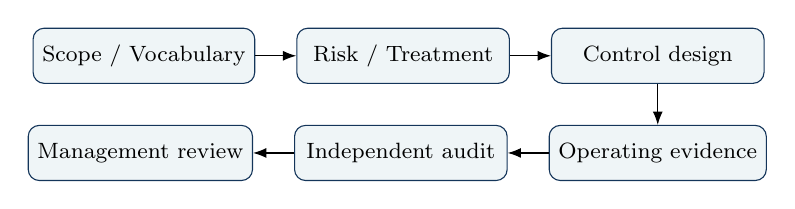
\begin{tikzpicture}[>=Latex,node distance=.52cm, every node/.style={font=\footnotesize},b/.style={draw=navy,fill=pale,rounded corners,minimum width=2.7cm,minimum height=.7cm,align=center}]
\node[b](a){Scope / Vocabulary};\node[b,right=of a](b){Risk / Treatment};\node[b,right=of b](c){Control design};\node[b,below=of c](d){Operating evidence};\node[b,left=of d](e){Independent audit};\node[b,left=of e](f){Management review};
\draw[->](a)--(b);\draw[->](b)--(c);\draw[->](c)--(d);\draw[->](d)--(e);\draw[->](e)--(f);
\end{tikzpicture}\end{center}
\section{Capstone case: multi-region financial services platform}
A 150-person engineering organization operates a cloud-hosted application platform, uses an offshore SaaS analytics provider and has limited control evidence. A new business partnership requires credible independent ISMS assessment. Students must define scope and supplier boundaries, identify twelve material scenarios, design risk treatments, justify 93 Annex A applicability decisions, implement five verifiable technical controls and run a mini internal audit.
\section{Capstone mandatory submissions}
\begin{enumerate}
\item Defined ISMS scope and material stakeholders/obligations with approval authority.
\item Risk criteria, minimum twelve assessed scenarios and named risk owners.
\item Statement of Applicability covering all 93 Annex A controls, plus any organization-specific controls.
\item Five control design/test packages, including one organizational, one people or physical, and two technical controls.
\item A complete audit plan, defensible samples, evidence register, at least three findings and corresponding action proposals.
\item A management review pack with residual exposure, metrics, decisions, resources and owners.
\end{enumerate}

\section{Competency rubric}
\small\rowcolors{2}{pale}{white}\begin{longtable}{p{.30\linewidth}p{.12\linewidth}p{.52\linewidth}}
\rowcolor{navy} \textcolor{white}{\textbf{Dimension}} & \textcolor{white}{\textbf{Weight}} & \textcolor{white}{\textbf{Strong submission}}\\
\endfirsthead
\rowcolor{navy} \textcolor{white}{\textbf{Dimension}} & \textcolor{white}{\textbf{Weight}} & \textcolor{white}{\textbf{Strong submission}}\\
\endhead
Source fidelity / terminology & 15\% & Separates 27001 requirements, 27002 guidance and local examples\\
Scope and risk rigor & 20\% & Consistent scenario/risk-owner/criteria chain\\
Applicability and SoA & 20\% & Defensible inclusion, non-applicability and current state\\
Engineering verification & 20\% & Risk-linked negative tests and reproducible evidence\\
Audit and independence & 15\% & Traceable criteria, populations and reviewed findings\\
Executive effectiveness & 10\% & Useful prioritization, resources, decisions and follow-up\\
\end{longtable}\normalsize

\section{Passing standard and progression}
Illustrative passing standard: at least 80/100 overall and no critical omission in scope, SoA, risk ownership, ethical testing or evidence integrity. Technical learners can then specialize in DevSecOps/AppSec; governance learners in enterprise risk and assurance; audit learners in sampling and conformity interpretation. This standard is a local training rubric, not an ISO certification examination.
\section{Instructor practical safety rules}
\begin{itemize}
\item Use synthetic secrets, intentionally vulnerable disposable applications and authorization-safe test environments.
\item Never test production infrastructure without explicit permission and coordinated change windows.
\item Do not publish personal data, internal policies, licensed standards or confidential evidence as class submissions.
\item Teach students to record uncertainty and untested populations rather than claim blanket compliance.
\end{itemize}

\clearpage\section*{Source and interpretation policy}
\addcontentsline{toc}{section}{Source and interpretation policy}
\textbf{Source editions:} ISO/IEC 27000:2018 (overview and vocabulary); ISO/IEC 27001:2022 (requirements and normative Annex A); ISO/IEC 27002:2022 corrected 2022-03 (control guidance). Specific clause identifiers are references to the supplied editions, not reproduced control text.\par
\textbf{Interpretation:} ``Source-grounded paraphrase'' describes a concept in the cited source. ``Engineering recommendation'' is a practical model, technology choice, owner, evidence example, frequency, template or scoring convention authored for this suite; it is not a claim that ISO prescribes that exact approach.\par
\textbf{Conformity:} Clauses 4--10 of ISO/IEC 27001 govern ISMS conformity. Applicability of controls is determined through risk treatment, with Annex A used as a completeness cross-check and exclusions justified in the Statement of Applicability (SoA). Source documents alone neither certify an ISMS nor prove control operating effectiveness.\par
\textbf{Source licensing:} Do not distribute or embed the licensed standard PDFs in repositories or distribute copied normative text. Review the editions, amendments, and certification scheme applicable to each assessment before relying on this work.\par
\end{document}
